Тестирование  на парах модельных изображений и на изображениях поверхностях реальных образцов.
\subsection{Образцы изображений}
\subsubsection{Модельные изображения}\label{mod_image}

Модель многослойного изображения.
Модельное изображение (рисунок \ref{pic:gray_mix}) получали из заданного количества слоёв псевдослучайных чисел; при этом каждый слой соответствует определённой пространственной частоте~\cite{pan_15}. Первый слой некоторого заданного исходного размера заполняется псевдослучайными значениями с равномерным распределением. Затем размер данного слоя увеличивается в два раза с помощью интерполирования бикубическим В-сплайном. Второй слой формируется аналогично первому, но перед увеличением его размера он складывается попиксельно с первым. Итеративно генерируются несколько слоёв, и на каждой итерации конечный размер изображения увеличивается в два раза. После генерации всех слоёв, проводится масштабирование и нормировка яркости в диапазоне от 0 до 255. Таким образом, имея начальный слой размером $4 \times 4$ пиксела, после проведения 8 итераций, получаем модельное изображение размером $1024 \times 1024$ пикселов.

Модель спекла (окрашенной поверхности). При создании модельного изображения спекла (рисунок \ref{pic:gray_mix}) (вторая серия) стояла задача создания изображения подобного экспериментально получаемым при фотографировании образца (рисунок \ref{pic:al_deform}). Для этого изображение ``заливали'' цветом, подобным по тону оттенку поверхности образца на экспериментально регистрируемых фотографиях. Затем в ``случайно'' заданных (по нормальному закону распределения) участках генерировали окружности (имитирующие капли распыляемой краски – пятна спекла), радиусом (0 до 10 пикселов), уровень (градация) серого которых задавался случайным образом.

Так же в качестве образцов брались наборы изображений из интернет ресурса ``Society for Experimental Mechanics (sem.org)'' описание текстур находится в таблице \ref{tab:set_image}, текстуры изображены на рисунке \ref{pic:gray_mix}.

\begin{figure}[h!]
\center{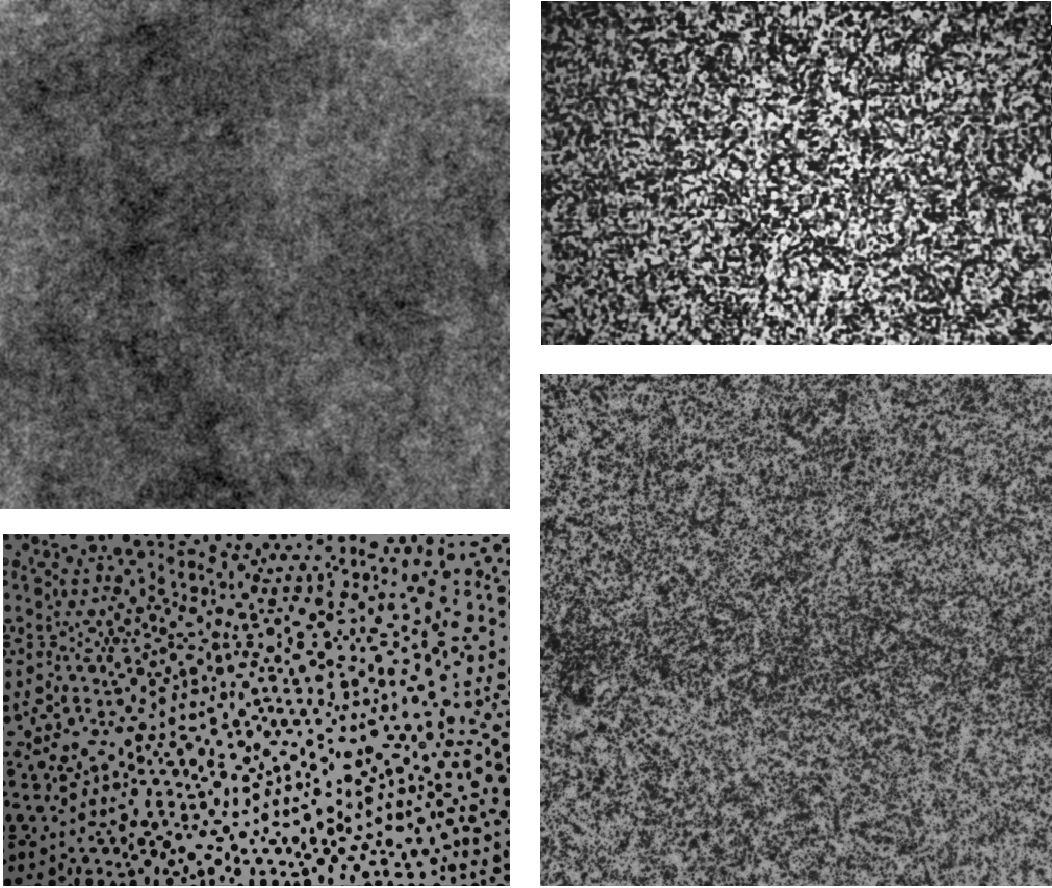
\includegraphics[width=0.9\linewidth]{gray_mix}}
\caption{Серия изображений: Модель многослойного изображения, Модель спекла, Высокий контраст, Prosilica Bin , Strain Gradient №1, Strain Gradient №2}
\label{pic:gray_mix}
\end{figure}

\begin{longtable}[h!]{|m{0.45\textwidth}|m{0.12\textwidth}|m{0.11\textwidth}|m{0.08\textwidth}|m{0.1\textwidth}|}
\caption{Описание модельных изображений}
\label{tab:set_image}
\\ \hline
Серия & Диапазон яркостей 	& Уровень шума & Сдвиг (px) &  Размеры \\ \hline
Модель многослойного изображения & 0-188 & Нет & 1-20 &  510x510 \\ \hline
Модель спекла & 0-188 & Нет & 1-70 &  512x512 \\ \hline
Высокий контраст & 10-240 & Низкий  & 0.1-1 & 487x325 \\ \hline
Prosilica Bin  & 10-156 & Низкий  & 0.1-1 & 487x325 \\ \hline
Strain Gradient №1 & 20-185 	& Средний  & 0.01-1 & 512x512 \\ \hline
Strain Gradient №2 & 30-225 	& Средний  & 0.01-1 & 512x512 \\ \hline
\end{longtable}

\subsubsection{Реальные отснятые изображения}

Реально отснятые изображения предоставлены сотрудником ИФПМ СО РАН. 

На первой серии (рисунок \ref{pic:al_deform}) изображён металлический образец из авиационного алюминиевого сплава Д16АТ нагружавшиеся на механической испытательной машине ИМАШ-2078 в условиях одноосного статического растяжения. Размеры предоставленных изображений 1920х1280 пикселей.
\begin{figure}[ht]
\center{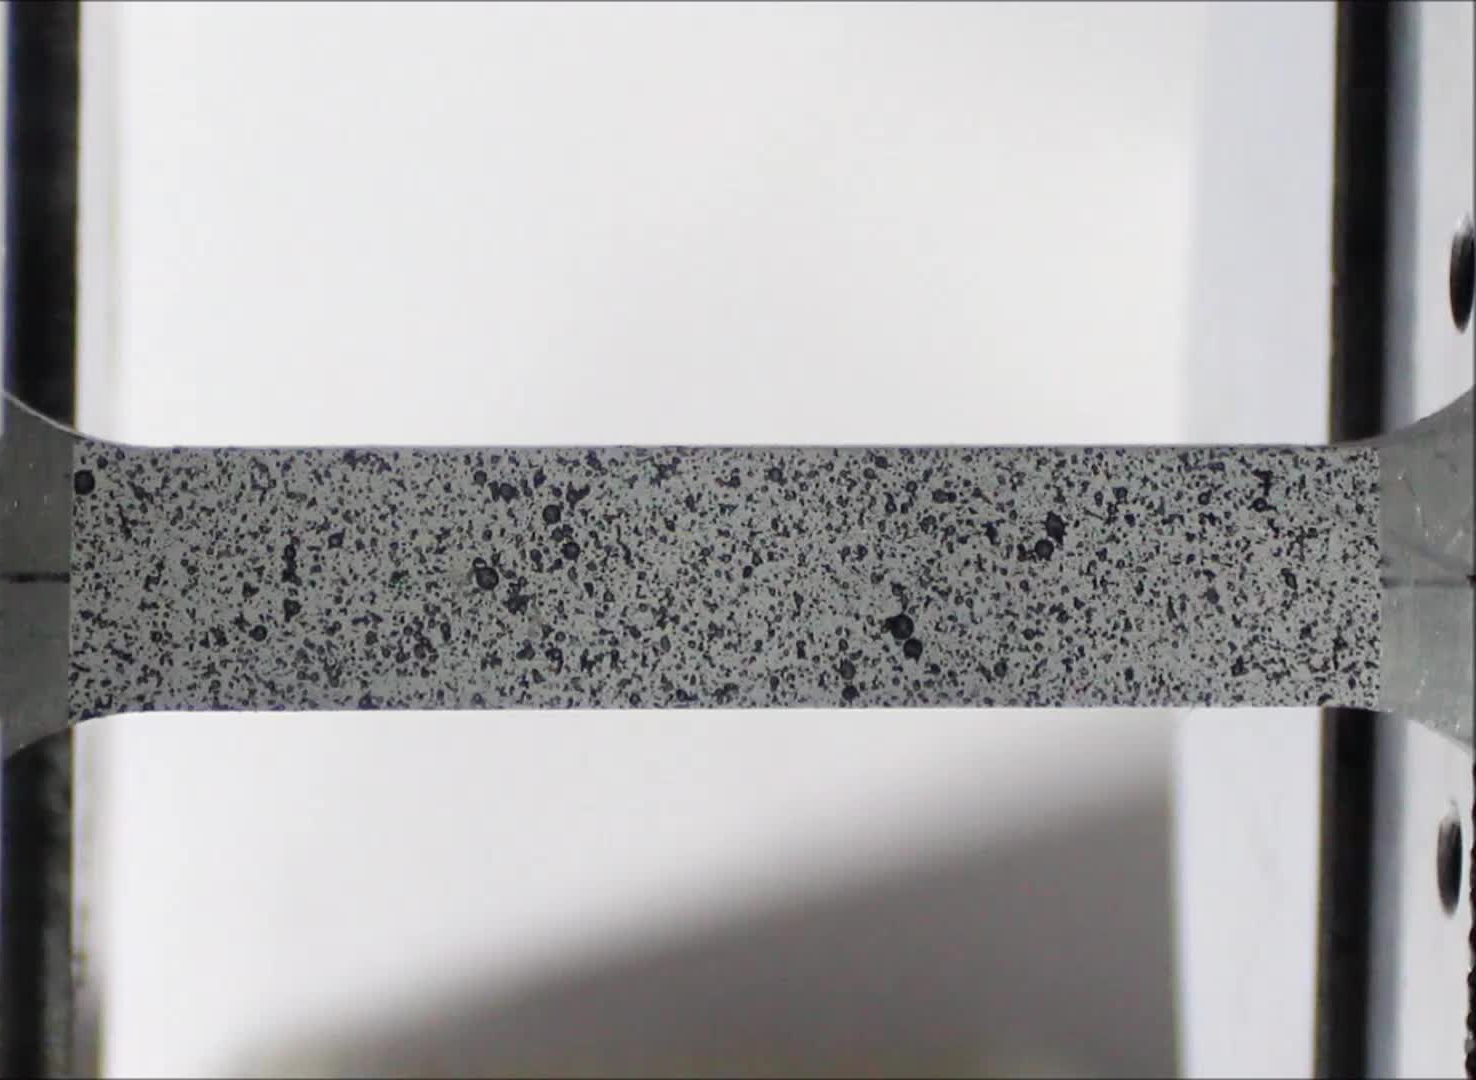
\includegraphics[width=0.6\linewidth]{al_deform}}
\caption{Растяжение пластины алюминия Д16АТ}
\label{pic:al_deform}
\end{figure}

На второй серии (рисунок \ref{pic:carbon_deform}) изображён углерод-углеродный композиционный материал. Образец испытывали на одноосное статическое растяжение на электро-механической машине Instron 5582 со скоростью перемещения подвижного захвата 0,3 мм/мин.
\begin{figure}[h!]
\center{\includegraphics[width=0.6\linewidth]{carbon_deform}}
\caption{Углерод-углеродный композиционный материал}
\label{pic:carbon_deform}
\end{figure}

Фотографирование поверхности осуществляли с помощью фотокамеры Canon EOS 550D, оснащённой длиннофокусным объективом Canon EF-S 100-400mm 1/4-5.6 IS.

\subsection {Оценка быстродействия}
Для проведения расчётов использовали ПЭВМ со следующими характеристиками:

Аппаратная составляющая:
\begin{itemize}
\item процессор Intel(R) Core(TM) i3 370M @ 2,4 ГГц, 64-бит;
\item оперативная память 4 Гб, 1067 МГц;
\item материнская плата Aspire 573
\item жёсткий диск SSD Smartbuy 120 Гб;
\item файловая система ext4, 107 Гб.
\end{itemize}
Программная составляющая:
\begin{itemize}
\item операционная система Linux Mint 3.19-18;
\item версия cmake 3.2.1;
\item версия QMake 3.0 \& Qt version 5.2.1;
\item версия компилятора gcc (Ubuntu 4.8.2-19ubuntu1) 4.8.2;
\item оболочка для среды рабочего стола Cinnamon 2.4.8.
\end{itemize}

Для исследования быстродействия и помехоустойчивости алгоритмов были использованы описанные ранее серии изображений.

\subsection{Тестирование программного обеспечения}
\subsubsection{Тестирование на модельных изображениях}
%Результатом работы ПО, как описано в * разделе, является векторное поле и поля деформации твёрдого тела представленное на рисунке \ref{pic:gray_set_out}.

Программное обеспечение будет тестироваться по модели белого ящика. Входные данные для тестирования описаны в разделе \ref{mod_image}, алгоритм работы описан на рисунке \ref{pic:shema_PO}.
 
Что определить погрешность работы программы, мы используем модельное изображение (рисунок \ref{pic:gray_mix} a), и сдвинем исходный рисунок по оси $x$ на один пиксель влево, по $y$ сдвиг отсутствует.
В таком случае, программа должна вычислить оптический поток, уловить этот общий сдвиг, а после построить поле деформации. Так как сдвиг по всему изображению равномерный то и деформация в этом случае отсутствует. Соответственно после расчёта программа вернёт нулевое поле (поле, заполненное нулями), все значения отличные от нуля, будут считаться ошибкой.

\subsubsection{Тестирование на экспериментально полученных изображения}
В данном разделе приведены результаты тестирования разрабатываемого программного обеспечения на изображениях поверхностей реальных образцов.

\begin{figure}
\centering
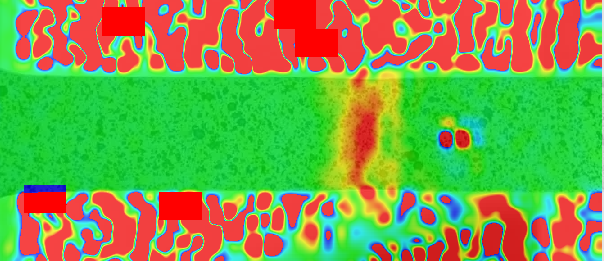
\includegraphics[width=0.7\linewidth]{images/al_strain}
\caption{Результат работы программы: верхний слой исходное изображение с 30\% альфа каналом, нижний слой -- поле деформации по оси $x$}
\label{fig:al_strain}
\end{figure}

\subsection{Исследование метода интерполяции}
В работе рассматривались три метода интерполяции:
\begin{itemize}
\item Билинейная
\item Бикубическая
\item Б-сплайн
\end{itemize}
Как сказано ранее, все существующие методы направлены либо на улучшение быстродействия, либо на шумостойкость. 
\begin{figure}
\centering
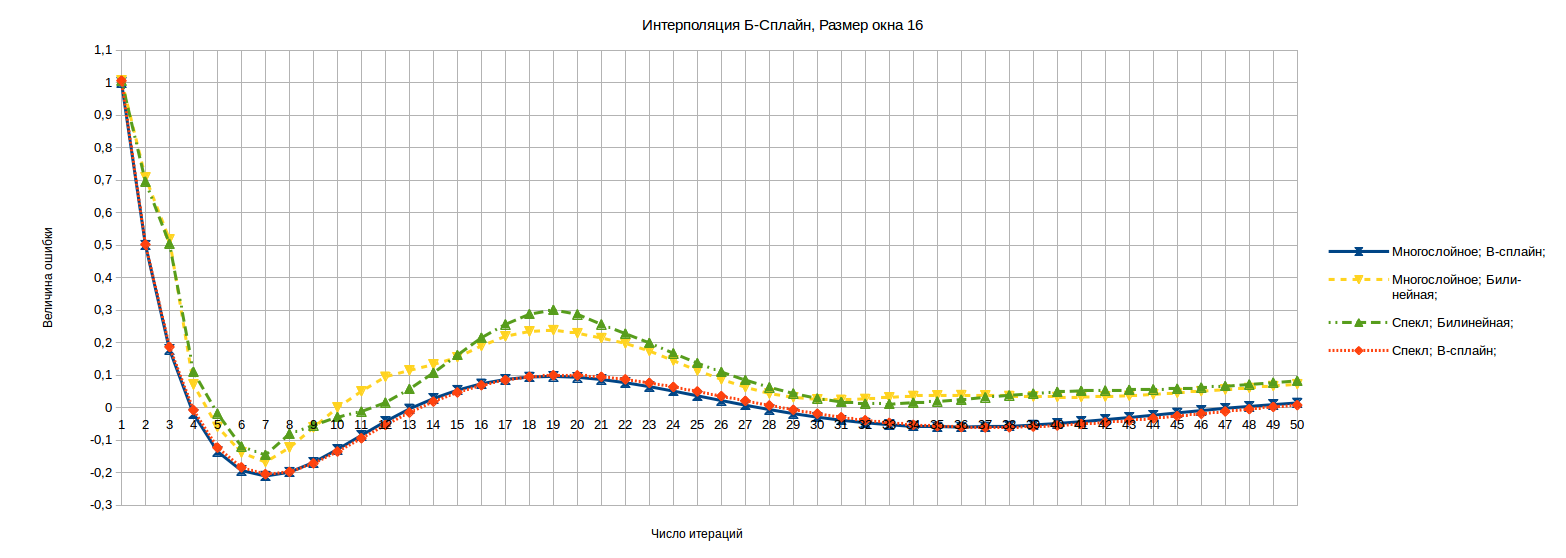
\includegraphics[width=0.8\linewidth]{images/inter_err}
\caption{Сравнение методов интерполяции}
\label{fig:inter_err}
\end{figure}
Соответственно, сравнятся будет уровень ошибки для разных реализаций, и время работы (рисунок \ref{fig:inter_err}).

Билинейный имеет наилучшее быстродействие, что очевидно и до этого. Но не так точен, как остальные методы интерполяции. Б-сплайн более точен, но и более медленный. Бикубическая интерполяция показывает схожий результат по точности с б-сплайном, только чуть лучше, но время работы значительно больше двух других методов. Исходя из выше сказанного, решено использовать для остальных тестирований б-сплайновую интерполяцию, т.к. он подобие золотой середины, с одной стороны более точный результат, с другой не такой медленный как бикубическая интерполяция. 
\subsection{Исследование размера окна поиска}

Тут некое вводное слово добавить. Оно показывает зависимость ошибки от размера окна корреляции. Так же нужно помнить, что реализованный алгоритм – локален и не может вычислить сдвиг больший чем заданное окно. Однако с увеличением размера окна, возрастёт число вычислений, соответственно время работы программы увеличивается, это зависимость представлена на рисунке \ref{fig:window_error}.
\begin{figure}
\centering
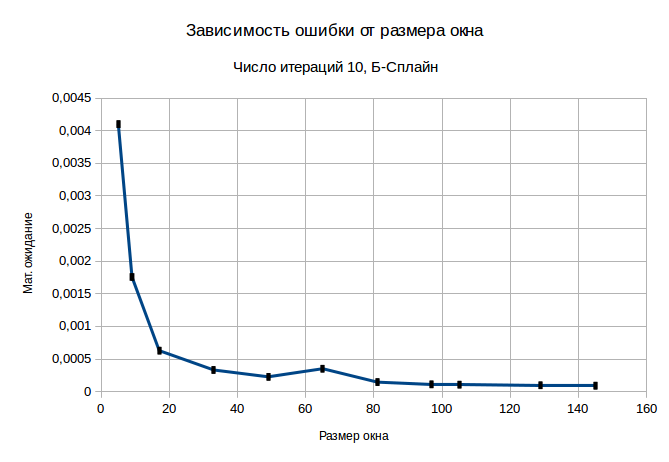
\includegraphics[width=0.7\linewidth]{images/window_error}
\caption{Величина ошибки в зависимости от размера окна корреляции}
\label{fig:window_error}
\end{figure}

\subsection{Исследование числа итераций}
\begin{figure}[h!]
\center{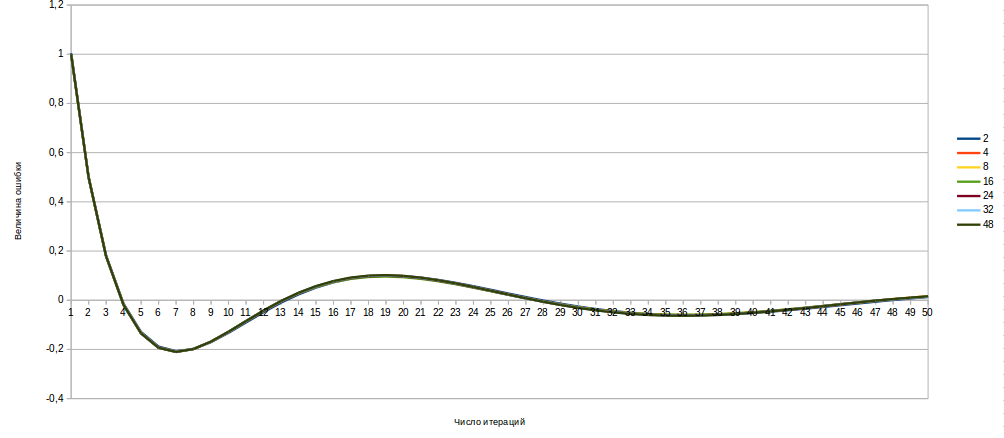
\includegraphics[width=0.6\linewidth]{images/window_size.png}}
\caption{Величина ошибки от числа итераций}
\label{fig:window_size}
\end{figure}

\begin{figure}[h!]
\center{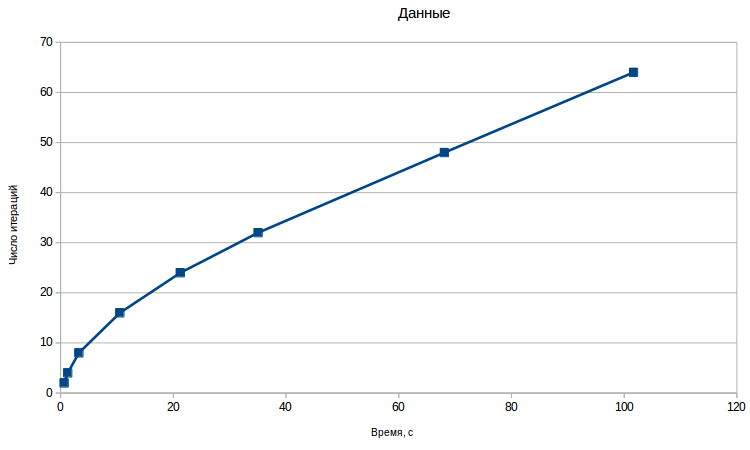
\includegraphics[width=0.6\linewidth]{images/window_time.png}}
\caption{Время работы программы, в зависимости от размера окна}
\label{pic:window_iter}
\end{figure}